\chapter{Análise técnica}\label{chp:Técnica}

\section{Determinando parâmetros}

Para modelar a  turbina respeitando os parâmetros fornecidos, consideramos 100 m de desnível fixo e, uma potência nominal de 100 MW.
Com base em uma pesquisa de turbinas com características de desempenho semelhantes, optamos por situar a turbina na situação descrita em \eqref{fig:esquema}, onde a barragem é vertical, possuindo um tubo que leva a água à turbina relativamente curto.

\begin{figure}[!h]
    \centering
    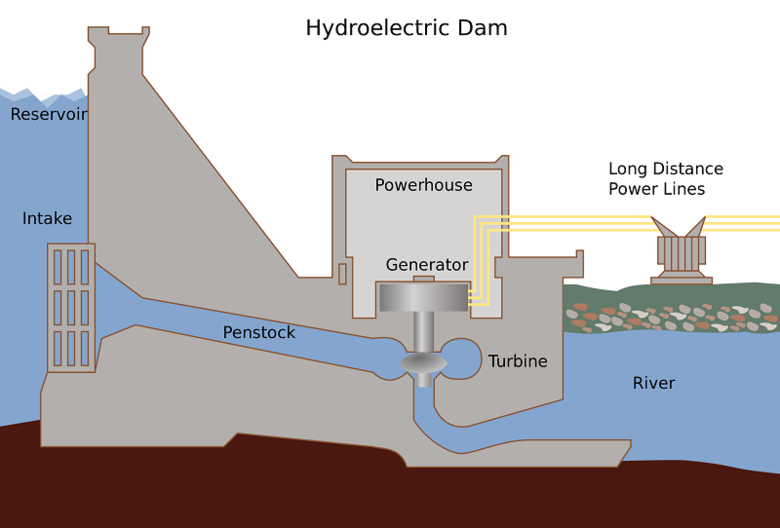
\includegraphics[width=0.6\textwidth]{figuras/scheme 2.png}
    \caption{Esquema do projeto}
    \label{fig:esquema}
\end{figure}

A partir desse esquema é possível equacionar o balanço de energia de uma linha de fluxo, partindo de um ponto na superfície do reservatário (ponto 1), com velocidade desprezível até um ponto na superfície do rio (ponto 2) também com velocidade desprezível. Ambos os pontos estão sujeitos à pressão atmosférica.

Utilizando a equação da energia para relacionar os parâmetros de carga hidráulica, carga da turbina e perdas generalizadas

\[\dfrac{p_1}{\rho}+\dfrac{v_1^2}{2}+gh_1 = \dfrac{p_2}{\rho}+\dfrac{v_2^2}{2}+gh_2 + gh_t + gh_l\]

Onde $h_t$ representa a carga entregue pela turbina e, $h_l$ a perda de carga agregada do sistema.

Assumindo as hipóteses descritas acima, ficamos com

\[(h1-h2) = h_t + h_l\]

\section{Modelando a turbina}

De acordo com \cite{hibbeler} podemos modelar de forma satizfatória a carga convertida pela turbina

\[h_t = \dfrac{U_2^2}{g} - \dfrac{U_2 Q cot(\beta_2)}{2\pi r_2 bg} - \dfrac{U_1 V_{t1}}{g}\]

Sendo $U_1 = \omega r_1$ e $U_2 = \omega r_2$ e

\[V_{t1} = kV_{r1} = \dfrac{kQ}{2\pi r_1 b}\]

Onde $Q$ é a vazão, $b$ a altura da turbina, $r_1$ é o raio interno das pás da turbina e $r_2$ o externo $k$ representando a parcela da vazão que possui velocidade tangencial à entrada da turbina, assumindo valores constantes entre $0$ e $1$ (levando em consideração a operação em uma condição estacionária) nesse caso será travado em $0,1$. Por fim, $\beta_2$ indica o ângulo entre a velocidade relativa de saída do fluido com a velocidade tangencial da pá , nesse caso será travado em $75\degree$.

\section{Modelando as perdas}

Utilizando-se da Lei de Poiseuille,

\[\Delta P = \dfrac{f}{2}\left(\dfrac{L}{D}\right)\rho V^2\]

onde $V$ é a velocidade média entre a entrada e a saída da turbina, em que ambas são dadas em termos da vazão.

\[V_1 = \dfrac{Q}{A_1} = \dfrac{4Q}{\pi d_1^2}\]

\[V_2 = \dfrac{Q}{A_2} = \dfrac{4Q}{\pi d_2^2}\]

Logo

\[V = \dfrac{2Q}{\pi}\left(\dfrac{1}{d_1^2} - \dfrac{1}{d_2^2}\right)\]

A partir dessa relação é possível obter uma aproximação razoável para todas as perdas envolvidas desde a entrada da barragem até a saída para o rio.

Para tanto, será tomada como parâmetro uma turbina da planta hidroelétrica de Furnas, cujas condições de operação nominal são, $90m$ de desnível, $150MW$ de potência mecânica e uma vazão de aproximadamente $190m^3/s$. O fator de atrito encontrado para os parâmetros fornecidos, a partir do diagrama de Moody foi $f = 0,008$.

Substituindo essas informações na equação da energia (em termos de potência específica)

\[hg = \dfrac{\dot{W}}{\dot{m}} + \dfrac{f}{2\rho}\left(\dfrac{L}{D}\right)\rho V^2\]

Isolando o termo $\left(\dfrac{L}{D}\right)$ é obtida uma relação que pode ser utilizada como parâmetro para a perda de carga do sistema a ser projetado, salvo as semelhanças que compartilha com a referência adotada.

\[\left(\dfrac{L}{D}\right) \approx 180\]

\section{Maximizando a função da eficiência}

Tratando se do rendimento da turbina na conversão da energia mecânica da água em potência de eixo, temos:

\[\eta = \dfrac{100\times10^6}{\rho gQh}\]

A vazão $Q$ é função implícita de $d1, d2, r1, r2, w$ e $b$.

Foi utilizada a função \textit{fmincon} do Matlab, para encontrar o mínimo do inverso da função da eficiência mostrada acima, maximizando-a, através da manipulação dos seis parâmetros que definem a vazão, sem deixar de respeitar as seguintes restrições:

\begin{itemize}
    \item $h_t \rho g Q = 100\times10^6$
    \item $r1<r2$
    \item A equação da energia deve ser conservada
\end{itemize}

Seguem os resultados dos parâmetros otimizados:

\[d1 = 7,3m \;\;  d2 = 7,3m  \;\; r1 = 4,2m \;\;  r2 = 8,37m  \;\;  \omega = 35,23rpm  \;\;  b = 2,74m\]

Gerando uma vazão de $Q = 115,2m^3/s$ e uma eficiência de $83,$

\section{Análise comparativa}

Tomando novamente uma turbina de furnas como referência, cujos dados são:

\[d1 = 5,2m \;\; d2 = 4,5m \;\; Q = 190m^3/s \omega = 150rpm \;\; \dot{W} = 152MW\]

Ficam evidentes determinadas semelhanças entre o modelo e a turbina real, dado que os diâmetros de entrada e saída estão próximos, e a vazão aparece maior nesse caso, juntamente com a velocidade, condizendo com a potência significativamente maior da referência tomada.

\section{Análise dimensional}

Será aplicada uma variação de $+50\%$ e $-50\%$ em cada parâmetro, enquanto os outros serão travados, em cada caso o valor da eficiência foi levado à zero se as restrições de projeto não forem atendidas (condicional no código) para facilitar a visualização, gerando os gráficos parâmetro x eficiência a seguir:

\begin{figure}[!h]
    \centering
    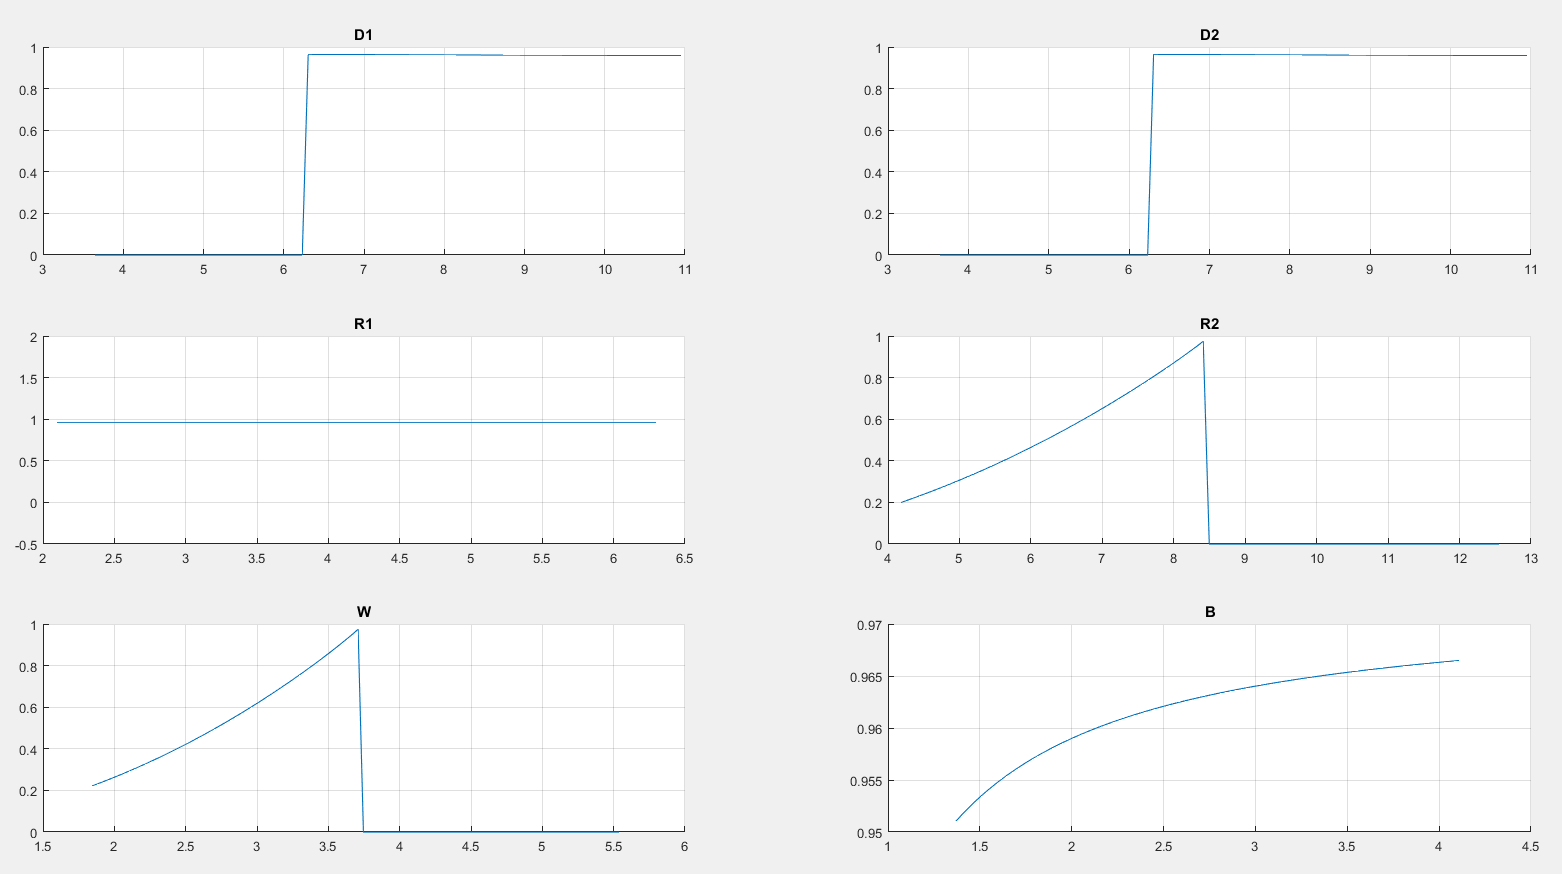
\includegraphics[width=1\textwidth]{figuras/bundled_graphs.jpg}
    \caption{Esquema do projeto}
    \label{fig:graphs}
\end{figure}

Em todos os gráficos, o ponto central é o escolhido pela otimização. Pode-se observar que o ponto central é aquele que maximiza a eficiência em todas as ocasiões, 